\documentclass[12pt]{report}
\usepackage[utf8]{inputenc}
\usepackage[T1]{fontenc}
\usepackage{graphicx}
\usepackage[export]{adjustbox}
\usepackage[a4paper, portrait, margin=1in]{geometry}
\usepackage[english]{babel}
\usepackage[utf8]{inputenc}
\usepackage[T1]{fontenc}
\usepackage{helvet}
\usepackage{etoolbox}
\usepackage{graphicx}
\usepackage{titlesec}
\usepackage{caption}
\usepackage{booktabs}
\usepackage{xcolor} 
\usepackage{titlesec}
\usepackage{setspace}
\graphicspath{ {./images/} }
\usepackage{pdfpages}

\usepackage{graphicx}
\usepackage[table,xcdraw]{xcolor}
%\usepackage{colortbl} 
%\usepackage{lscape}
%\usepackage{float}
% Please add the following required packages to your document preamble:
%\usepackage[table,xcdraw]{xcolor}
% Beamer presentation requires 
%\usepackage{longtable}
% Note: It may be necessary to compile the document several times to get a multi-page table to line up properly




% Set chapter and section headings formatting
\titleformat{\chapter}[display]{\normalfont\fontsize{10}{19}\bfseries\centering}{\chaptertitlename\ \thechapter}{0.5em}{\MakeUppercase}
\titleformat{\section}[block]{\normalfont\fontsize{12}{14.4}\bfseries}{\thesection}{1em}{\MakeUppercase}
\titleformat{\subsection}[block]{\normalfont\fontsize{12}{14.4}\itshape}{\thesubsection}{1em}{\MakeUppercase}

% Set figure and table captions formatting
%\captionsetup[figure]{font={small,normal}}
%\captionsetup[table]{font={small,normal}}

% Set footnote text size
\renewcommand{\footnotesize}{\fontsize{9}{11}\selectfont}


\usepackage[square,sort,comma,numbers,super]{natbib}

 

\usepackage{caption}
\usepackage{float}
\graphicspath{ {./Images/} }
\makeatletter
\patchcmd{\@maketitle}{\Large \@title}{\fontsize{16}{19.2}\selectfont\@title}{}{}
\makeatother
\date{}    

\usepackage{amsmath} % for math environments and operations
\usepackage{bm}      % for bold symbols in math mode

\begin{document}







\doublespacing
\thispagestyle{empty}
\pagenumbering{roman}
\vspace*{0.3cm}
\begin{center}
\textbf{ \Large
Dust, Gas, and Metallicities of Cosmologically Distant Lens
Galaxies \\
}
\vspace*{2cm}
\textbf{Phys 4310 - Capstone} 
\vspace*{2cm}

By \\
\vspace*{1cm}
\textbf{Blake T Johnson}

\textbf{}
\vspace*{2cm} \\
Under the guidance of

\textbf{Dr. Xinyu Dai}
\vspace*{2cm}
\begin{center}

\includegraphics[max width=0.25\textwidth]{Images/University_of_Oklahoma_seal.svg.png}
\end{center}

\textbf{Homer L Dodge Department of Physics and Astronomy, \\ University of Oklahoma, Oklahoma \\ NOVEMBER, 2023}
\end{center}



\newpage
\tableofcontents
%\listoffigures
%\listoftables






\newpage
\pagenumbering{arabic}


\chapter{INTRODUCTION}

My capstone project was to analyze the X \textemdash ray observations of 10 gravitational lenses, HE 0047 \textemdash 1756, QJ 0158\textemdash 4325, SDSS 0246 \textemdash 0805, HE 0435 \textemdash 1223,
SDSS 0924+0219, SDSS 1004+4112, HE 1104 \textemdash 1805, PG 1115+080,
Q 1355 \textemdash 2257, and Q 2237+0305, to measure the X \textemdash ray absorption
between images, the metallicity, and the dust \textemdash to \textemdash gas ratio of the lens galaxies. The objective is to measure how much dust and gas are in the interstellar medium of different galaxies. We used images from the Chandra X \textemdash ray telescope to obtain our data.\\

During my time in capstone, I collected 124 images from Chandra relating to our 10 observations. I loaded them into the school computer and then reprocessed the images to get a clear image. Then I created a psf file for the images and created a Sherpa script for three different energy levels in order to help me run a spectrum on the X-rays.\\

In this paper I will discuss the objectives of our research and why it is important, how I plan to make our measurements and why it is effective, the process taken up to this point for the research, and what we have left to do.


\chapter{Our Objective}
The objective of our research is to determine the dust, gas, and metalicities in the interstellar medium. We want to calculate the ratio of dust to gas, obtain more research in this area, and obtain a better understanding of the activities in galaxies.\\

It is important to understand the interstellar medium (ISM) and the intergalactic medium (IGM). We use the ISM and IGM in studying many areas of astronomy, specifically in star and galaxy formation and studying evolution. Measuring the extinction by dust in the ISM is also important so that we can make corrections when using high redshift standard candles. These corrections will help us correctly determine the physical properties of sources and images. We measure extinction laws by comparing the spectra of reddened and un-reddened stars of the same spectral type so it is important for us to be able to correct for the dust and gas in our measurements.


\chapter{How lensing helps to measure dust and gas}
Gravitational lensing happens when an extremely massive object - in our research a galaxy - causes the curvature of spacetime. The path of light flows through spacetime and appears visibly bent (much like light bends through a lens). The large mass that causes the bending of the spacetime is called a gravitational lens.\cite{Information@eso.org_2020}\\

Einstein explained in his general theory of relativity that time and space are two sides of the same coin. He called the coin "spacetime." Very large objects cause space to curve. Gravity is the curvature of the spacetime. Light travels through spacetime and curves when spacetime curves. Gravitational lensing is a very large example of this theory\cite{Information@eso.org_2020}.

As light approaches these large galaxies, the light is curved in different directions around the galaxy. To an observer on the other side of the galaxy, it appears that there are multiple light sources, not just a single light.

\begin{figure}[H]
    \centering
    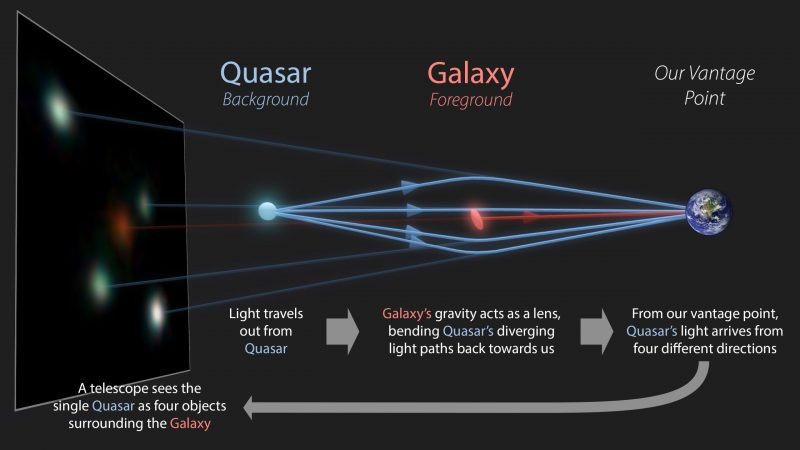
\includegraphics[width=0.5\textwidth]{Images/Lensing.jpeg}
    \caption{gravitational lens\cite{earthsky.com_2021}}
    \label{fig:gravitational lens}
\end{figure}

Different rays of light cross through the lensed galaxy at different points. The amounts of dust and gas in the galaxy vary depending on the position. For instance, there is less gas on the outskirts of the galaxy than there is at the center of the galaxy. As the rays pass through the galaxy they get obstructed by the gas. This causes a shift in their spectrum. Since each light ray passes through the lens at a different position, they each are interfered with differently by the gas. Each light ray has a different spectrum shift based on how much gas is interfering with it.\\

From an observer on Earth, we view these bent lights as separate images. We can then take each image's spectrum and analyze its redshift to determine how much dust and gas are interfering with it. Then we can analyze the dust, gas, and metalicities at different points in the galaxy.


\chapter{The Research}
My specific part of this research involved preparing to analyze 10 different observations. The data I used came from the Chandra X-ray telescope. I then loaded these images into the University computer and then cleaned the images up to prepare them to be analyzed. I also prepared all the scripts necessary to run the spectral images. The next step is to run the spectrums for each image. I will discuss the steps I took in the next sections.
\subsection{Obtaining the Data}
The 10 observations that we are analyzing are quasars that are lensed through galaxies. The Chandra X-ray telescope had already imaged these observations. So the first step in my research was gathering the data. I submitted a request to Chandra for the data on these images and they emailed me the files.\\
Once I had the files I loaded them into the University computer and sorted the files based on their observations. There were several images that they sent for each image. I ended up with a total of 124 images total after I gathered all 10 observations. 
\subsection{Reprocess}
Chandra sent a primary and secondary file (data distributions) for each image. Each folder had an evt2.fits file attached. Evt2.fits files are the physical photos that can be viewed in DS9. I needed to get one clean photo for each image. So I reprocessed the primary and secondary files to get a new clear evt2.fits. "The chandra \textunderscore repro script takes the data from these data distributions and creates a new bad pixel file, a new level=2 event file, and a new level=2 Type II PHA file (grating data only) along with the appropriate per-order and per-arm ARF and RMF files.\cite{Chandra_2023}"\\
Reprocessing was simple. Chandra has a simple script that does all the work. I just executed the script for each image. Now I had a single repro file for each image with a repro\textunderscore evt2.fits image which combines the primary and secondary image. This is the photo that we want to use for our analysis. 

\subsection{Creating a PSF image}
Once the repro file was set up I created a psf.fits inside each repro file. Psf stands for point spread function. A point spread function is the infinite-resolution and infinite-signal-to-noise flux distribution from a point source on the detector, after passing through optics, dust, atmosphere, etc. \cite{Doe1_2023}. So it is important for us to apply this to our images.\\
"Chandra produces sharper images than any other X-ray telescope to date; and therefore, provides an opportunity for high-angular and spectral resolution studies of X-ray sources. Crucial to these studies is the knowledge of the characteristics of the PSF. The observed Chandra PSF is smeared with the blur introduced to the High-Resolution Mirror Assembly (HRMA) PSF by a combination of the telescope dithering motion, the limited size of detector pixels, and detector effects.\cite{Doe1_2023} The blurring of the Chandra PSF is introduced by the HRMA PSF, the aspect, the limited size of detector pixels and detector effects. Simulating the HRMA PSF using ChaRT is the first step in obtaining a good model of the Chandra PSF for a given observation. The shape and size of the HRMA PSFs vary significantly with source location in the telescope field of view (FOV), as well as with the spectral energy distribution of the source. The image quality is best in a small area centered about the optical axis. In fact, the mirrors were designed to produce images with better than one arc-second resolution; in particular to concentrate better than 85\% of the energy at 0.277 keV within a 1 arcsec diameter\cite{Chandra_2023}"\\

\subsection{Creating a full, hard, and soft image}
Once I applied the psf to each repro file I then needed to create images specifically focused on different energies. Chandra recommends that we filter the event files on energy before beginning the analysis. The energy ranges that I used were specifically given to my by Dr. Dai. I created images, from the evt2.fits image, that focuses on energies ranging from 200-2000, another from 2000-8000, and one from 200-8000. I created new fits for each one of these energy ranges using the 'dmcopy' command. This command creates a new evt2 file that only includes data in the specified energy range. The fits with energies from 200-2000 is labeled "soft," the fits with energies ranging from 2000-8000 is "hard," and the fits with the full range is labeled "full." These will be used in analyzing the shift.\cite{Doe_2023}

\subsection{creating Sherpa texts}
Once the full, soft, and hard photos of all 124 images were complete I was ready to run Sherpa. Sherpa is a command through a program called Ciao that pulls the spectrum of the images. Ciao is Chandra's software used to analyze the images.\\

Sherpa is designed to do several things with your data. "Sherpa is the CIAO modeling and fitting application. It enables the user to construct complex models from simple definitions and fit those models to data, using a variety of statistics and optimization methods. It lets you
\begin{itemize}
    \item fit 1-D data sets (simultaneously or individually), including:
spectra, surface brightness profiles, light curves, general ASCII arrays
    \item fit 2-D images/surfaces in the Poisson/Gaussian regime
    \item visualize the data with Matplotlib and DS9
    \item visualize the data with Matplotlib and DS9
    \item access the internal data arrays
    \item build complex model expressions
    \item import and use your own models
    \item choose appropriate statistics for modeling Poisson or Gaussian data
    \item import new statistics, with priors if required by analysis
    \item visualize a parameter space with simulations or using 1-D/2-D cuts of the parameter space
    \item calculate confidence levels on the best-fit model parameters
    \item choose a robust optimization method for the fit: Levenberg-Marquardt, Nelder-Mead Simplex or Monte Carlo/Differential Evolution
    \item perform Bayesian analysis with Poisson Likelihood and priors, using Metropolis or Metropolis-Hastings algorithm in the MCMC (Markov-Chain Monte Carlo)
    \item and use Python to create complex analysis and modeling functions, build the batch mode analysis or extend the provided functionality to meet the required needs." \cite{Doe1_2023}

I want to use Sherpa to fit 1-D image for Spectra, to visualize the data with Matplot lib, and to use Python to create complex analysis and modeling functions.

\end{itemize}

We ran into some issues with Ciao during the semester. The University needed to update Ciao for me to be able to run my script. It took the University longer than expected to update the software and get me access. In the meantime, I created the scripts needed to run the spectroscopy. I want to run spectroscopy for each of the evt2.fits files, hard, soft, and full. I created a text file for each one of these and labeled it accordingly, Sherpa \textunderscore full.txt, Sherpa \textunderscore soft.txt, Sherpa \textunderscore hard.txt

\chapter{Next Steps}
Once the University gets Ciao updated and gives me permission to access it, I can start running spectrum for all the images and then analyze the information. The Sherpa scripts are all ready, it is a matter of copying and passing them into Ciao. Although I have not run Ciao before, I did ask a grad student who has Ciao on his personal computer to run an example of the program. I have put that example in Appendix A so you can see what the spectrum should look like.
\chapter{Conclusion}
I have organized the files so that, in the event I am unable to complete my research before graduation, any upcoming undergraduate can copy the files into their own log in and be able to pick up where I left off. I hope that the University can get ciao operational in the next week or so. This will allow me one more semester to try and complete my work and analysis. Either way, all of the data is organized and ready for analysis.

\appendix
\chapter{Q \textunderscore 1355 Spectrum}

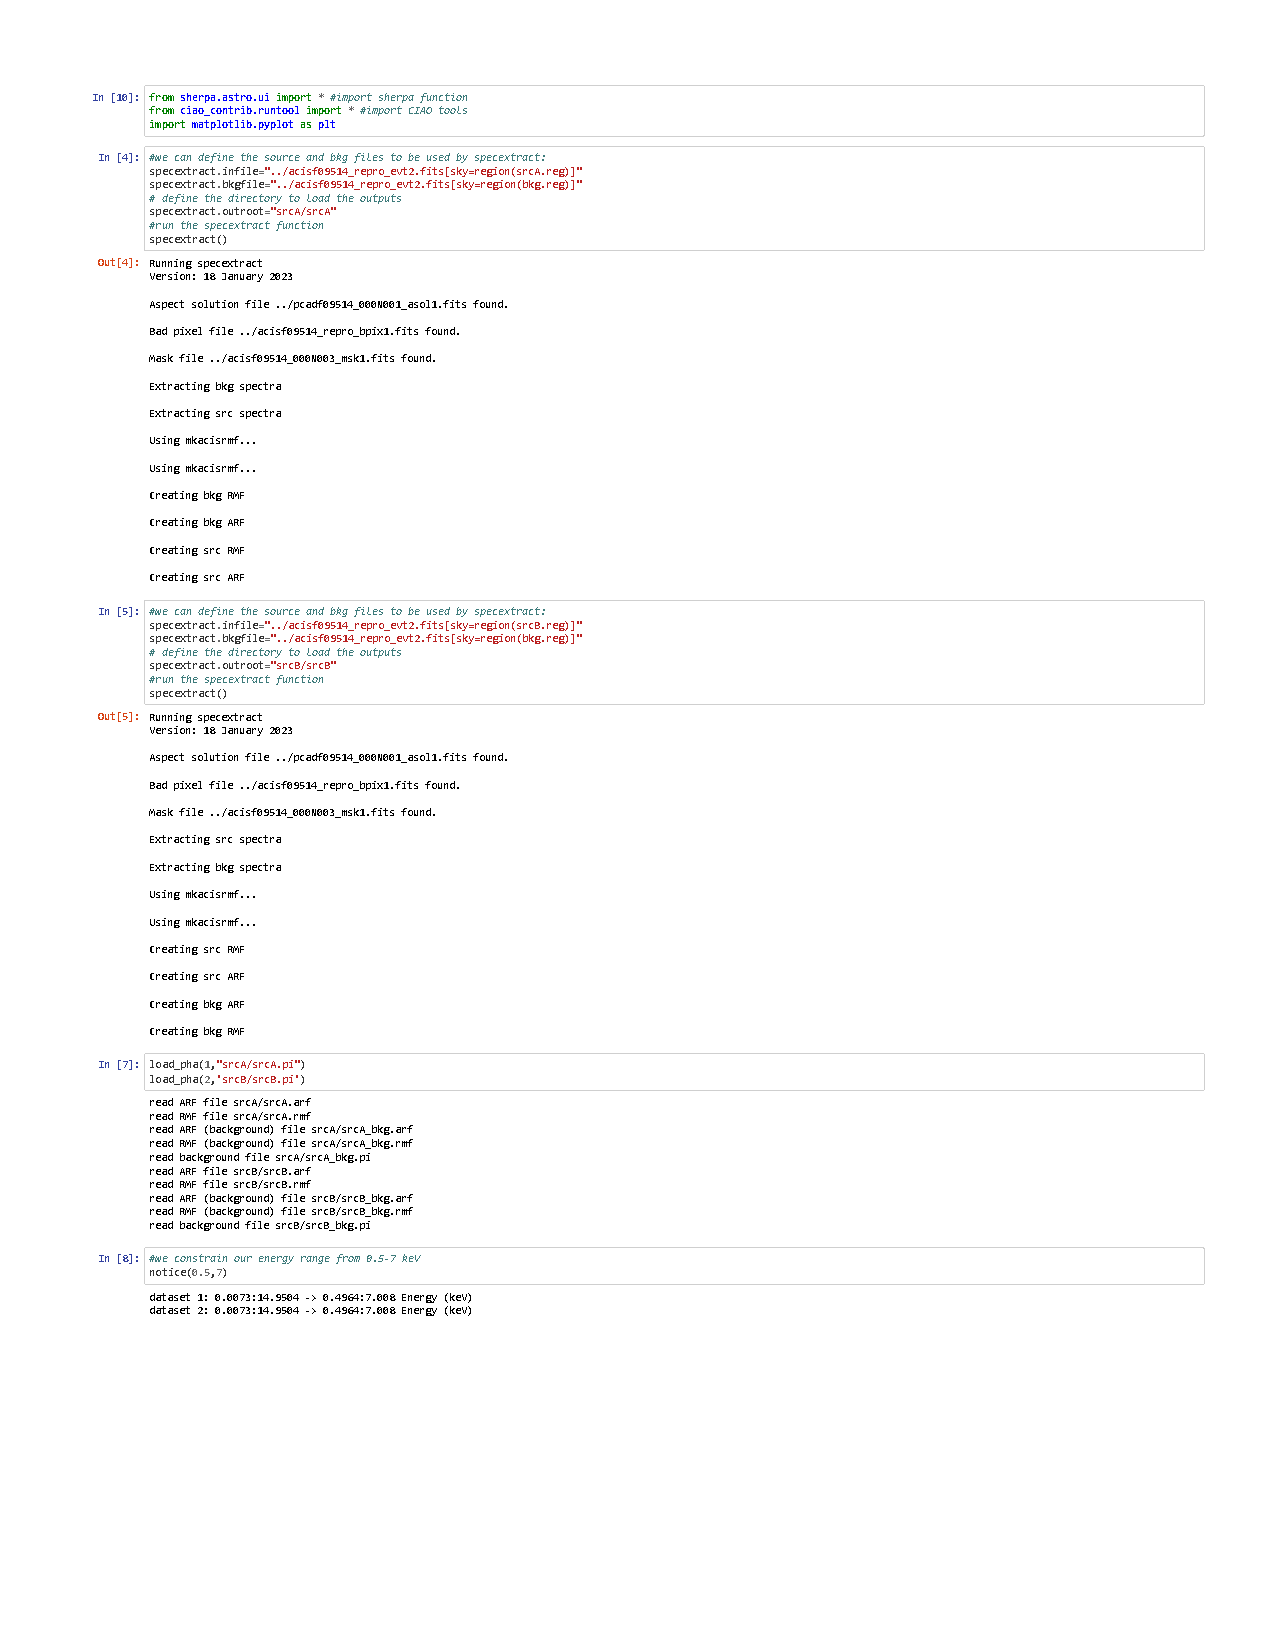
\includegraphics[scale=0.75,page=1]{Images/blake_src1.pdf}
\includegraphics[scale=0.75,page=2]{Images/blake_src1.pdf}
\includegraphics[scale=0.75,page=3]{Images/blake_src1.pdf}
\includegraphics[scale=0.75,page=4]{Images/blake_src1.pdf}
\includegraphics[scale=0.75,page=5]{Images/blake_src1.pdf}



\bibliographystyle{ieeetr}
\bibliography{references}
\clearpage
%appendix


\end{document}